\documentclass{article}
\usepackage{pgfplots}

\begin{document}

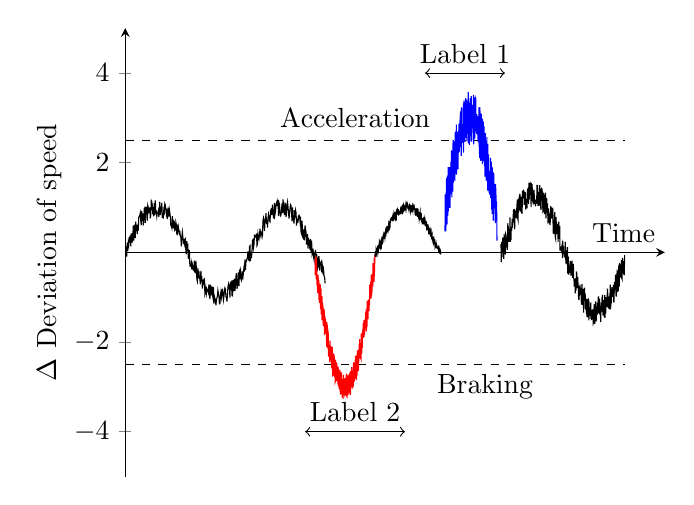
\begin{tikzpicture}
\begin{axis}[
    xlabel={Time},
    ylabel={$\Delta$ Deviation of speed},
    ymin=-5,
    ymax=5,
    xmin=0,
    xmax=27,
    axis lines=middle,
    xtick=\empty,
    ylabel style={at={(axis description cs:-0.1,0.5)},rotate=90,anchor=south}, % Shift the y label here
]  
% Dotted threshold lines
\addplot[dashed, domain=0:25] {2.5};
\addplot[dashed, domain=0:25] {-2.5};

% Signal with noise: Modified to be continuous and longer
\addplot[color=black, domain=0:10, samples=400] {sin(deg(x)) + 0.2*rand}; % Regular signal with noise
\addplot[color=red, domain=9.5:12.5, samples=400] {3*sin(deg(x)) + 0.3*rand}; % Signal above 2.5 threshold with noise labeled as Layer 1
\addplot[color=black, domain=12.5:15.8, samples=200] {sin(deg(x)) + 0.1*rand}; % Regular signal with noise
\addplot[color=blue, domain=16:18.6, samples=360] {-3*sin(deg(x)) + 0.6*rand}; % Signal below -2.5 threshold with noise labeled as Layer 2
\addplot[color=black, domain=18.8:25, samples=400] {1.3*sin(deg(x)) + 0.3*rand}; % Regular signal with noise

% Horizontal arrows with labels
\draw[<->] (axis cs: 15,4) -- (axis cs: 19,4) node[midway,above] {Label 1};
\draw[<->] (axis cs: 9,-4) -- (axis cs: 14,-4) node[midway,above] {Label 2};


% Annotations
\node at (axis cs: 11.5,3) {Acceleration};
\node at (axis cs: 18,-3) {Braking};

\end{axis}
\end{tikzpicture}

\end{document}
